\documentclass[a4paper]{jpconf}
\usepackage{xurl}
\usepackage{float}
\usepackage{amsmath}
\usepackage{hyperref}
\usepackage{subcaption}
\usepackage{amssymb}
\usepackage{graphicx}
\usepackage{mathtools}
\usepackage{xcolor}
\DeclarePairedDelimiter\ceil{\lceil}{\rceil}
\DeclarePairedDelimiter\floor{\lfloor}{\rfloor}

\makeatletter
\newcommand*\bigcdot{\mathpalette\bigcdot@{.5}}
\newcommand*\bigcdot@[2]{\mathbin{\vcenter{\hbox{\scalebox{#2}{$\m@th#1\bullet$}}}}}
\makeatother

\begin{document}
\nocite{*}
\title{Review of `Phase seperation explains a new class of
self-organized spatial patterns in ecological systems' by Liu et al.}

\author{L Post}

\address{MSc in Physics and Mathematics, University of Amsterdam, NL}

\ead{\url{leanderpost@gmail.com}}

% \begin{abstract} This report is not really serious enough for an abstract but my template requires one :)
%     \textbf{Content: } I'll discuss the paper `Spatiotemporal Pattern Formation in Neural Fields' by G.B. Ermentrout et al. I'll mostly fill in some gaps in the analysis, reproduce the numerical simulations, and critique some aspects that I find lacking. \textbf{Results: } The intuition provided by the article seems correct, and most of the analysis too. However, figure 4.1 is not reproducible with the parameters provided, with errors in several aspects. \textbf{Conclusion: } The paper is very useful in explaining the phenomena, but is hard to check.
% \end{abstract}

\section{Introduction}

The paper I'm reviewing is `Phase seperation explains a new class of self-organized spatial patterns in ecological systems' by Liu et al. The paper shows a novel way that biological systems can show phase-seperation. The classic go-to explanation of patterns in biological systems has been Turing bifurcations for a long time. The paper gives the example of mussel-aggregation. With a rather simple model, fitted to observations, this model gives rise to a partial differential equation that is similar to the Cahn-Hilliard equation that one encounters in the physics of fluids. This partial differential equation has been studied extensively, both by phycisists and mathematicians. Casting biological (mostly ecological) systems into this framework is therefore useful, as a lot of theory can be directly applied. 
\section{Brief outline}
I'll start by deriving the partial differential equation, which consists of a non-linear second order diffusive term, which comes from a density-dependend velocity, which gives rise to a density-dependend Fick's law. The model also takes longer range interactions into account, which gives rise to a fourth order diffusive term. I'll show how to conclude that we should get a fourth order term as the only reasonable next order. Then I'll add something the paper hasn't done explicitly, I'll do a linear stability analysis of the homogeneous state with constant mussel-density with an accompanying bifurcation diagram. Then I'll add some remarks about existence of solutions. Finally, I'll note some things that seemed a bit off about the paper and have some concluding remarks.
\section{Density-dependend diffusion}
\begin{figure}[h!]
    \centering
    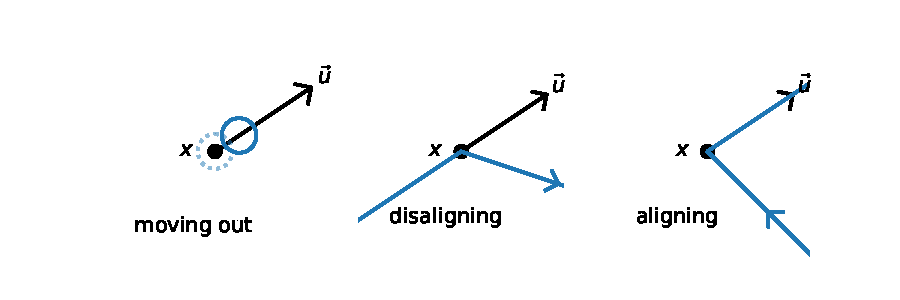
\includegraphics[width=0.8\linewidth]{/home/leander/OneDrive/master/YearTwo/MB/project/code/change.pdf}
    \caption{Cartoon of the time derivative of $P(x,\vec u,t)$}
\end{figure}
The paper used a density-dependent diffusion term. This term can be derived by considering a continuous random walk model with density and flux given by:
\[\begin{aligned}
M(x,t) &= \oint_{S^n} P(x,\vec u,t)d\vec u\\
\vec J(x,t) &=V(M) \oint_{S^n} P(x,\vec u,t)\vec ud\vec u
\end{aligned}\]
Here, $P(x,\vec u,t)$ is the probability density of finding a particle (mussel) at position $x$, at time $t$, going in direction $\vec u$. The model is quite similar to the one introduced in the lecture. By integrating over all directions, we find the density at some position and time, which we'll call $M$. By multiplying by $\vec u$ and integrating over all directions, we get the flux at some position and time. The integrals are over the unit sphere. The source \cite{schnitzer} has constant $V$, but we'd like to bake in the $M$-dependence. Note that $\Omega(n)$ is just the integral over the unit sphere, so that's the surface of the $n$-sphere, which has an explicit form. In our $3D$ case, this will of course just be $4\pi$. Now conservation of mass together with the dynamics of the system gives:
\[\begin{aligned}
P_t(x,\vec u,t) &= -\nabla(V(M)P(x,\vec u,t))\cdot \vec u -\tau P(x,\vec u,t)+\frac{\tau }{\Omega(n)}\oint_{S^n}P(x,\vec u',t)d\vec u'\\
&=\underbrace{-\nabla(VP)\cdot \vec u}_{\text{particles moving out}}-\underbrace{\tau P}_{\text{disaligning}}+\underbrace{\frac{\tau M}{\Omega(n)}}_{\text{aligning}}
\end{aligned}\]
We can explain the terms as follows, the mussel-density that moves away from $x,t$ is the mussels that come in minus the mussels that move out. The gradient of $VP$ gives the this difference, and the dot product with $u$ ensures we look at the mussels moving out in the right direction. Next, the constant $\tau$ gives the rate at which mussels change direction. In principle this could be density-dependent, but we don't need it to be for the model. I'll have a remark about that later. Lastly, the integral term represents the probability of a particle aligning. The integral over the sphere represents all the directions, and $\tau/\Omega(n)$ gives the probability of aligning. We're not too interested in transient effects, and want to go to a (quasi)-stable state. Then we can investigate the solutions to $P_t=0$:
\[\begin{aligned}
    0 &= -\nabla(VP)\cdot \vec u-\tau P+\frac{\tau M}{\Omega(n)}\\
    \implies P &= \frac{-\nabla(VP)\cdot \vec u}{\tau}+\frac{M}{\Omega(n)}
\end{aligned}\]
% \[
% P = \frac{-\nabla(VP)\cdot \vec u}{\tau}+\frac{M}{\Omega(n)}
% \[
Now let's assume we are close to equilibrium, then we can write $P = M/\Omega(n)$ (particles go in all directions with equal probability), which gives:
\[
P = \frac{-\nabla(V M)\cdot \vec u}{\tau \Omega(n)}+\frac{M}{\Omega(n)}
\]
We want an expression for $\vec J$, so we can multiply by $\vec u$, integrate over $S^n$ and multiply by $v(M)$ to get:
\[
J = V(M)\oint_{S^n}P\vec ud\vec u = -V(M)\oint_{S^n} \frac{\nabla (VM)\cdot \vec u }{\tau \Omega(n)}\vec ud\vec u +V\frac{M}{\Omega(n)}\oint_{S^n} \vec u d\vec u
\]
Now we assume $VM$ is approximately independent of $\vec u$, which is an assumption we'll elaborate on later. Then we can use the fact that $\vec u$ is an odd function to see that the second integral vanishes, and we can use the fact that $\vec u \vec u$ is an $n\times n$ tensor with trace one ($\vec u\cdot \vec u=1$), so by symmetry, the integral should be  $\Omega(n)/n$ times the identity. For example, in our $S^2$ case:
\[\begin{aligned}
\int_{S^2}\vec u\vec ud\vec u&=\int_0^\pi\int_0^{2\pi} (\sin\phi\cos \theta,\sin\phi\sin \theta)^T(\sin\phi\cos \theta,\sin\phi\sin \theta)d\theta d\phi\\
&=\int_0^\pi\int_0^{2\pi}\sin\phi \begin{pmatrix}\cos^2\theta&\cos\theta\sin\theta\\ \sin\theta\cos\theta&\sin^2\theta \end{pmatrix}d\theta d\phi\\
&=\int_{0}^\pi\sin\phi \begin{pmatrix}\pi&0\\ 0&\pi \end{pmatrix} d\phi=\begin{pmatrix}2\pi&0\\ 0&2\pi \end{pmatrix}
\end{aligned}\]
Which is indeed $\Omega(2)/2$ times the identity. 

Combining these facts, we get:
\[
J = -V\frac{\nabla(VM)}{n\tau} = -V\frac{V\nabla M+M\nabla V}{n\tau} =-\frac{V(V+MV_M)}{n\tau} \nabla M
\]
Or if we write $f(M)=V(V+MV_M)$, we get $J  = -f(M)\nabla M$. 
\section{High order diffusion}
\begin{figure}[h!]
    \centering
    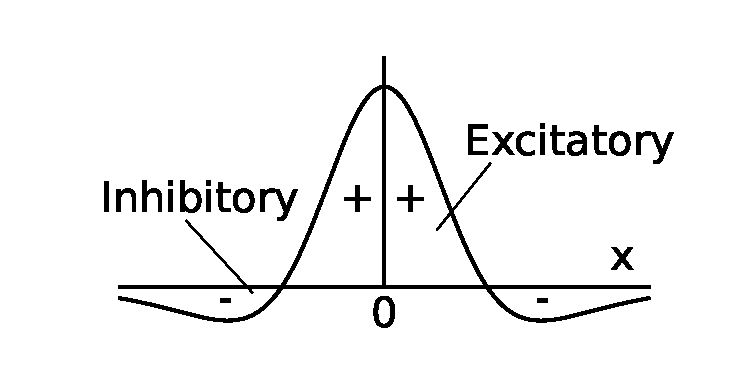
\includegraphics[width=0.4\linewidth]{/home/leander/OneDrive/master/YearTwo/MB/project/code/kernel.pdf}
        
    \caption{Cartoon of interaction kernel}\label{kernel}
\end{figure}
Here I'll show that if we want to include non-local effects and stabilize the second order term, but want to stay in the land of differential equations, it makes sense to add a fourth order differential term. For this section, I'll assume that $M$ is $C^4$ at least and that the moments of $w$ exist.
We'd like to keep non-local effects into account. To get an intuition for what kind of terms we can expect, consider the following integro-differential equation, which we will reduce to a differential equation:
\[
M_t(x',y') = \int_{X}w(x,y)M(x'-x,y'-y)dxdy
\]
In Mathematical Neuroscience, this is a classic way to get a system to have non-local interactions, the kernel tells us how much a particle at position $x$, influences the rest of the system. At $x'$, the system at $x$ contributes $w(x'-x)$. Here $X$ is our domain. We can taylor $M$ to get:
\[
M_t(x',y') = \int_{X}w(x,y)\left[M(x',y')+M_x(x',y')x+M_y(x',y')y+\dots\right]dxdy
\]
When $w$ has a small support, or is quickly vanishing, this taylor makes a lot of sense, as $M$ only matters locally in that case, as bits further away get multiplied by kernel $w$ that is small at that point! Now assuming the system is isotropic, we get an even $w$, so the odd moments vanish. Adopting the notation $w_{ij}=\int_X w(x,y) x^iy^idxdy$, we get:
\[\begin{aligned}M_t(x,y) &= w_{00} M(x,y)+\frac{w_{20}}{2}M_{xx}+\frac{w_{02}}{2}M_{yy}+\frac{w_{40}}{24}M_{xxxx}\\
&+\frac{w_{22}}{12}M_{xxyy}+\frac{w_{04}}{24}M_{yyyy}+h.o.t.
\end{aligned}\]
Now again by isotropy, and assuming the domain is larger than the support of $w$, we can write $w_{40}=w_{22}=w_{04}$. Then, note that $\Delta(\Delta M)=M_{xxxx}+2M_{xxyy}+M_{yyyy}$, so we can write:
\[
M_t = w_{00}M+\frac{w_{20}}{2}\Delta M+\frac{1}{24}w_{40} \Delta(\Delta M)
\]
Next, to have conservation of mussels, the kernel should average to $0$, otherwise a presence of mussels removes/adds mussels, and since we don't consider death of birth, this is not the case, therefore $\int_X w(x,y)dxdy = w_{00}=0$. Then we're left with something familiar:
\[
M_t = D_1\Delta M+D_2\Delta(\Delta M) = \nabla \cdot (D_1\nabla M+D_2\nabla(\Delta M))
\]
\section{Full model}
We already found an expression for our first order derivatives of the flux, so we can combine the results to get:
\[
M_t = D\nabla \cdot \left(\frac{V(V+MV_M)}{n\tau} \nabla M -\kappa \nabla (\Delta M)\right) = D\nabla \cdot \left(f(M) \nabla M -\kappa \nabla (\Delta M)\right)
\]
Interestingly, $V>0$ (it's the velocity), so the zeros of $f$ are the same as the zeros of $V+MV_M$. Measurement has shown that it is statistically founded to pick a quadratic $V(M)$. So this is precisely what we'll assume. Then, as we have a quadratic determining the zeros in the biologically well-defined regime $V>0$, we get at most two zeros. \\
We'd like to rescale the problem to make it look similar to the Cahn-Hilliard equation, and we do this by setting $m = \sqrt\frac{a}{c}M$ and $\beta = \frac{b}{\sqrt{ac}}$, then we get:
\[\begin{aligned}
 f(M)&=\frac{1}{n\tau } \left(a \sqrt\frac{c}{a}^2 m-\beta\sqrt{ac}\sqrt\frac{c}{a}m+c\right)\left( 3a \sqrt\frac{c}{a}^2 m-2\beta\sqrt{ac}\sqrt\frac{c}{a}m+c\right)\\
&=\frac{c^2}{n\tau}(m^2-\beta m+1)(3m^2-2\beta m+1):= \frac{c^2}{n\tau }g(m)
\end{aligned}\]
This imposes that $\beta^2<4$, since the first term $m^2-\beta m+1>0$, so the discriminant $\beta^2-4$ should be smaller than $0$, to not have $V(m)=0$ anywhere. Now all the terms in the differential equation have one unscaled $M$ term left, so we can rescale all those simultaneously to get:
\[
m_t = D\nabla \cdot \left(\frac{c^2}{n\tau}g(m) \nabla m -\kappa \nabla (\Delta m)\right)
\]
Now we can set $D_0 = \frac{c^2}{n\tau}D$ and $\kappa_1 =\frac{n\tau}{c^2}\kappa$, then we get:
\[
m_t = D_0\nabla \cdot \left(g(m) \nabla m -\kappa_1 \nabla (\Delta m)\right)
\]
If we now define $P$ such that $\nabla P=g(m)\nabla M$, it's clear that 
\[\begin{aligned}P(m)&=\int g(m) \, dm=
\int (m^2 - \beta m + 1)(3m^2 - 2\beta m + 1) \, dm \\
&=\int (3m^4 - 5\beta m^3 + 2\beta^2 m^2 + 4m^2 - 3\beta m + 1) \, dm\\
&= \frac{3}{5}m^5 - \frac{5\beta}{4}m^4 + \frac{2\beta^2 + 4}{3}m^3 - \frac{3\beta}{2}m^2 + m + C\end{aligned}\]
does just that, since $\nabla P=P_M\nabla M = g(m)\nabla M$. Then we can write:
\[
m_t = D_0\nabla^2(P(m)-\kappa_1\Delta m)
\]
At this point, we've come quite close to the form of the Cahn-Hilliard equation. The difference is that we have a quintic, while CH requires a cubic. It turns out this doesn't matter too much, as long as $P$ looks like a double well potential: with 2 minima, and 1 maximum, which then is in the middle. By the way we constructed $g(m)$, and thereby $P(m)$, we know that it has $3$ zeroes, therefore $P$ will have the required 3 zeroes.
$Q$, the antiderivative of $P$ or the free energy/potential, will therefore have $3$ extrema. For large $m$, we get $Q=\int Pdm\sim \frac1{10}m^6$, which indicates that we will have a $\bigcup$ shaped function if we zoom out enough. Then necesarily, we get $2$ minima, and 1 maximum (actually it could also have two saddles and a minimum, but we can choose $C$ such that this never happens).This is the condition for Cahn-Hilliard, and therefore, we can use the existence results from [boek over CH] to see that we indeed get a solution. 


\section{Linear stability analysis}
We'd like to see if the uniform state $m_0$ is stable, to predict for which values we can expect bifurcations. To do so, we use linear stability analysis. 

\[
m_t = D_0\nabla^2(P(m)-\kappa_1\Delta m)
\]
Following a similar analysis to [book over CH], we find:
setting $m(x,t)=n(x,t)+m_0$, with $n(x,t)$ a small perturbation on top of $m_0$, we get:
\[
n_t = m_t = D_0\nabla^2(P(m_0+n)-\kappa_1\Delta n)
\]
Expanding $P$, we get:
\[
P(n+m_0) = P(m_0)+P'(m_0)n+O(n^2) = P(m_0)+g(m_0)n+O(n^2)
\]
Amazing, now let's toss the constant, as we're going to take the derivative with respect to $x$, and let's also toss anything order $n^2$ or higher. Then to first order, we can write:
\[
n_t  = D_0\nabla^2(g(m_0)n-\kappa_1\Delta n)
\]
Assuming a square environment, with Neumann boundary conditions (mussels can't leave our square box), we can apply a Fourier series to find that for a mode $\phi(k_x,k_y)=\exp(\lambda t)\sin(k_xx)\sin(k_yy)$ (where I anticipate that the Neumann BC give only sines): 
\[\begin{aligned}
\lambda\phi(k_x,k_y) &= D_0(-k_x^2-k_y^2)(g(m_0)\phi(k_x,k_y)-\kappa_1 (-k_x^2-k_y^2) \phi(k_x,k_y))\\
&= D_0(-k_x^2-k_y^2)(g(m_0)-\kappa_1 (-k_x^2-k_y^2) )\phi(k_x,k_y)
\end{aligned}\]
If we write $\Omega=[0,L_x]\times[0,L_y]$, we get that pairs of numbers $(l_x,l_y)$ define a mode $\sin(k_xx)\sin(k_yy)$ by $\sin(k_xL_x)=0$ and $\sin(k_yL_y)=0$. This happens when $k_xL_x =\pi l_x$ and $k_yL_y=\pi l_y$. So we can write: $\phi(l_x,l_y)=\sin\left(\frac{\pi l_x}{L_x}x\right)\cos\left(\frac{\pi l_x}{L_x}x\right)$. 
Now we'd like to see when we get unstable nodes. Note how we decoupled space and time by going to spatial frequency and time, so our modes simply grow/decay exponentially:
\[
\lambda = D_0(-k_x^2-k_y^2)(g(m_0)-\kappa_1 (-k_x^2-k_y^2) )
\]
So if we want to see patterns, we need some growing nodes, this happens when:
\[
D_0(-k_x^2-k_y^2)(g(m_0)-\kappa_1 (-k_x^2-k_y^2) )>0
\]
So when:
\[
-K^2(C+\kappa_1K^2)>0\implies -K^2(g(m_0)/\kappa_1+K^2)>0
\]
This is now a simple polynomial in $K^2$, which is the sum of the earlier wavenumbers $k_x^2+k_y^2$. We know that $\kappa_1$ is positive, so this is a $\bigcap$ shaped parabola. Furthermore, we see that we always have at least one zero, at $K^2=0$, however, its maximum, the fastest growing mode, is between $0$ and $-g(m_0)/\kappa_1$ now, so at $K^2_*=\max(-g(m)/(2\kappa_1),0)$ if we take the restriction that $K^2_*$ be positive in mind. Note this is not nessesarily a sum of two integers squared, but that doesn't matter too much if the system size is large enough. Now with this in mind, we can use python to get the bifurcation diagram of the "fastest growing mode", $K_*$, with $m_0$ as bifurcation parameter, see figure \ref{bif_beta_m0}. 
Like expected, there is a range where the homogeneous state is not stable. In this regime, we can expect patterns, as the theory tells us there is a stable solution, and we've just figured out that it can't be the uniform one. 

\begin{figure}[h!]
    \centering
    \begin{subfigure}[t]{0.5\textwidth}\centering
        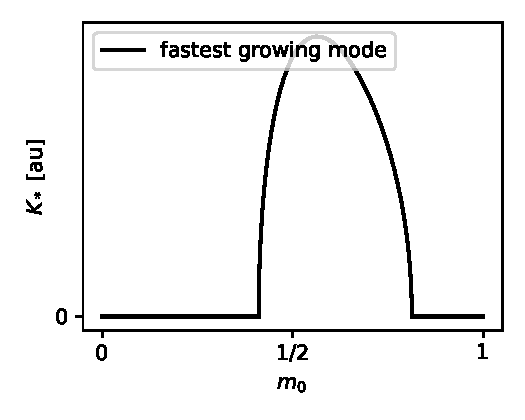
\includegraphics[width=1\linewidth]{/home/leander/OneDrive/master/YearTwo/MB/project/code/fastest_mode.pdf}
        % \caption{}\label{fastest_mode}
    \end{subfigure}\hfill
    \begin{subfigure}[t]{0.5\textwidth}\centering
        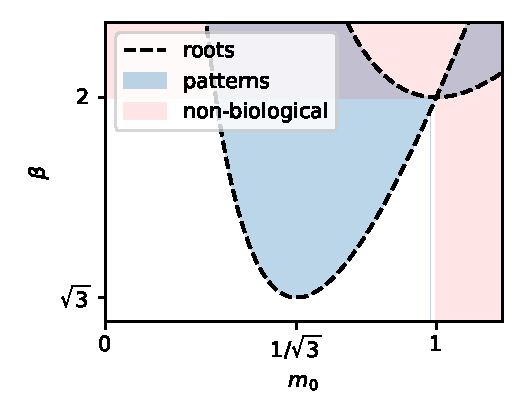
\includegraphics[width=1\linewidth]{/home/leander/OneDrive/master/YearTwo/MB/project/code/bif_beta_m0.pdf}
        
        % \caption{}\label{bif_beta_m0}
    \end{subfigure}
    \caption{(left) Plot of the fastest mode, as a function of $m_0$, the average density. This is for $\beta=1.83$, which you get when using $a=  2.3$, $b = 2.19$ and $c = 0.62$, as given in the paper. Note the units are arbitrary, and can be scaled with $\kappa_1$. (right) Bifurcation diagram in two parameters, the shaded area gives the parameter combinations where uniform solutions are not stable.}\label{bif_beta_m0}
\end{figure}

For a completer picture, we can now look at the zeros of $g(m)$, because these give rise to unstable solutions. We have the roots of $g(m)$:
\[
\begin{aligned}
g^{-1}(0) =  \left\{\frac{1}{2}\left(\beta \pm \sqrt{\beta^2 - 4}\right) ,\frac{1}{3}\left(\beta \pm \sqrt{\beta^2 - 3}\right)\right\} \\
\end{aligned}
\]
Plotting these gives the bifurcation diagram in figure \ref{bif_beta_m0}.
Where the paper says that patterns emerge when $\sqrt 3<\beta<2$ is satisfied, this is a little bit inaccurate, as also above $\beta=2$ patterns emerge, it's just that those values are non-biological, as $\beta>2$ implies negative velocity for some density of mussels (whatever that may mean). 

\section{Discussion}
In general, the paper was very readible, the supplementary material was good, and I could find very little errors. A small error is in the bifurcation diagram in figure $S1$, where the axis label says we're talking about $M$, while this should be the scaled and dimensionless $m$. \\


\section{Conclusion}

\section*{References}
\bibliographystyle{iopart-num}
\bibliography{curtu03}


\end{document}